% ---------------------------------------------------------------------------
% What QCD lets out of the house. A free particle must be a colour singlet:
% the allowed combinations are those in which the colours cancel, a quark
% with an antiquark (3 x 3bar contains 1), three quarks or three antiquarks
% (3 x 3 x 3 contains 1), and the rarer multiquark states and glueballs; a
% lone quark, a diquark (3 x 3 = 3bar + 6, no singlet) or a q q qbar carry
% colour and are forbidden. The Lund string makes only the first row's
% mesons and baryons: its ends are quarks, antiquarks and diquarks.
% ---------------------------------------------------------------------------
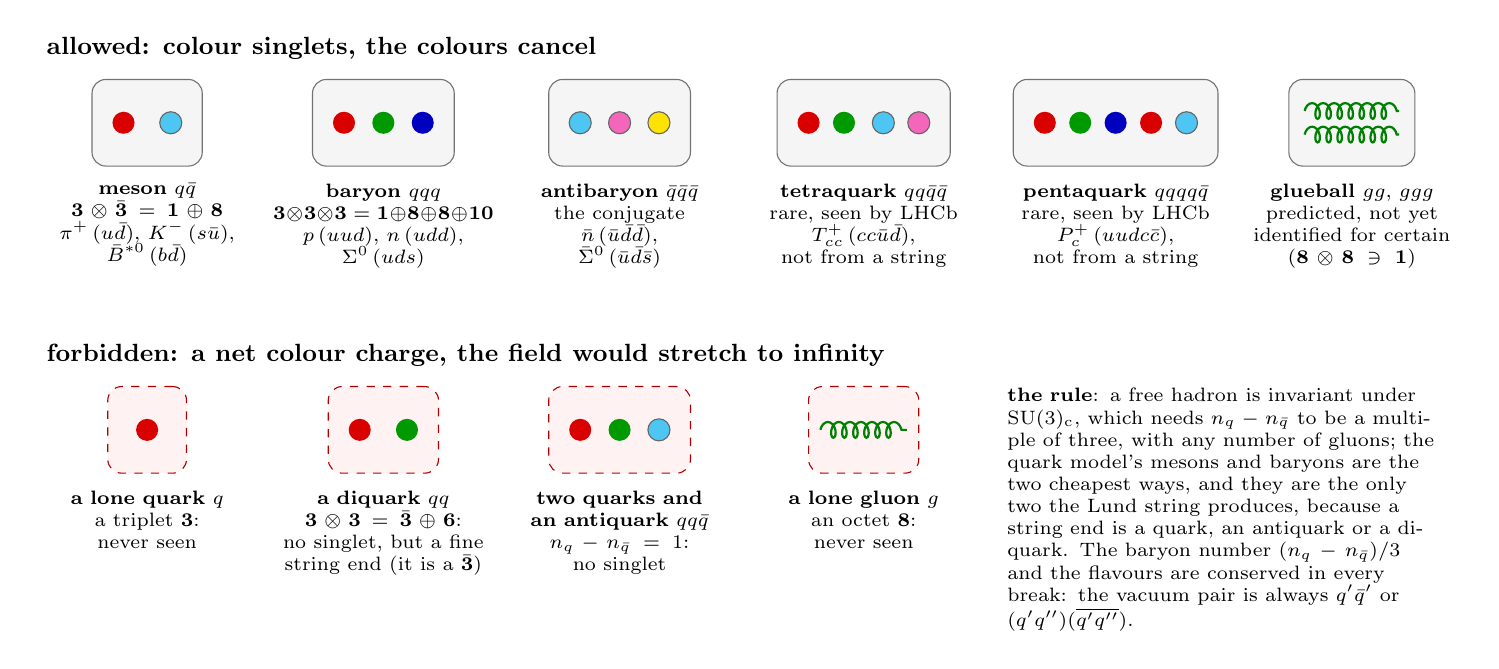
\begin{tikzpicture}[x=1cm,y=1cm,
  every node/.style={font=\footnotesize},
  cr/.style={circle,inner sep=0pt,minimum size=2.8mm,fill=red!85!black},
  cg/.style={circle,inner sep=0pt,minimum size=2.8mm,fill=green!60!black},
  cb/.style={circle,inner sep=0pt,minimum size=2.8mm,fill=blue!75!black},
  ar/.style={circle,inner sep=0pt,minimum size=2.8mm,fill=cyan!70,draw=black!60,line width=0.4pt},
  ag/.style={circle,inner sep=0pt,minimum size=2.8mm,fill=magenta!60,draw=black!60,line width=0.4pt},
  ab/.style={circle,inner sep=0pt,minimum size=2.8mm,fill=yellow!85!orange,draw=black!60,line width=0.4pt},
  bag/.style={rounded corners=5pt,draw=black!55,fill=black!4,minimum height=11mm,inner sep=2pt},
  bad/.style={rounded corners=5pt,draw=red!70!black,dashed,fill=red!5,minimum height=11mm,inner sep=2pt},
  lab/.style={font=\scriptsize,align=center,text width=2.8cm},
  rule/.style={font=\scriptsize,align=left},
  head/.style={font=\small\bfseries}]
% ---------------- allowed --------------------------------------------------------------------------
\node[head,anchor=west] at (-0.5,3.55) {allowed: colour singlets, the colours cancel};
% meson at x = 0.9
\node[bag,minimum width=14mm] at (0.9,2.6) {}; \node[cr] at (0.6,2.6) {}; \node[ar] at (1.2,2.6) {};
\node[lab,anchor=north] at (0.9,1.95) {\textbf{meson} $q\bar q$\\ $\mathbf3\otimes\bar{\mathbf3}=\mathbf1\oplus\mathbf8$\\ $\pi^+\,(u\bar d)$, $K^-\,(s\bar u)$,\\ $\bar B^{*0}\,(b\bar d)$};
% baryon at x = 3.9
\node[bag,minimum width=18mm] at (3.9,2.6) {}; \node[cr] at (3.4,2.6) {}; \node[cg] at (3.9,2.6) {}; \node[cb] at (4.4,2.6) {};
\node[lab,anchor=north] at (3.9,1.95) {\textbf{baryon} $qqq$\\ $\mathbf3\otimes\mathbf3\otimes\mathbf3=\mathbf1\oplus\mathbf8\oplus\mathbf8\oplus\mathbf{10}$\\ $p\,(uud)$, $n\,(udd)$,\\ $\Sigma^0\,(uds)$};
% antibaryon at x = 6.9
\node[bag,minimum width=18mm] at (6.9,2.6) {}; \node[ar] at (6.4,2.6) {}; \node[ag] at (6.9,2.6) {}; \node[ab] at (7.4,2.6) {};
\node[lab,anchor=north] at (6.9,1.95) {\textbf{antibaryon} $\bar q\bar q\bar q$\\ the conjugate\\ $\bar n\,(\bar u\bar d\bar d)$,\\ $\bar\Sigma^0\,(\bar u\bar d\bar s)$};
% tetraquark at x = 10.0
\node[bag,minimum width=22mm] at (10.0,2.6) {}; \node[cr] at (9.3,2.6) {}; \node[cg] at (9.75,2.6) {}; \node[ar] at (10.25,2.6) {}; \node[ag] at (10.7,2.6) {};
\node[lab,anchor=north] at (10.0,1.95) {\textbf{tetraquark} $qq\bar q\bar q$\\ rare, seen by LHCb\\ $T_{cc}^+\,(cc\bar u\bar d)$,\\ not from a string};
% pentaquark at x = 13.2
\node[bag,minimum width=26mm] at (13.2,2.6) {}; \node[cr] at (12.3,2.6) {}; \node[cg] at (12.75,2.6) {}; \node[cb] at (13.2,2.6) {}; \node[cr] at (13.65,2.6) {}; \node[ar] at (14.1,2.6) {};
\node[lab,anchor=north] at (13.2,1.95) {\textbf{pentaquark} $qqqq\bar q$\\ rare, seen by LHCb\\ $P_c^+\,(uudc\bar c)$,\\ not from a string};
% glueball at x = 16.2
\node[bag,minimum width=16mm] at (16.2,2.6) {};
\draw[decorate,decoration={coil,aspect=0.6,segment length=1.4mm,amplitude=1mm},green!50!black,thick] (15.6,2.45) -- (16.8,2.45);
\draw[decorate,decoration={coil,aspect=0.6,segment length=1.4mm,amplitude=1mm},green!50!black,thick] (15.6,2.75) -- (16.8,2.75);
\node[lab,anchor=north] at (16.2,1.95) {\textbf{glueball} $gg$, $ggg$\\ predicted, not yet\\ identified for certain\\ ($\mathbf8\otimes\mathbf8\ni\mathbf1$)};
% ---------------- forbidden ------------------------------------------------------------------------
\node[head,anchor=west] at (-0.5,-0.35) {forbidden: a net colour charge, the field would stretch to infinity};
\node[bad,minimum width=10mm] at (0.9,-1.3) {}; \node[cr] at (0.9,-1.3) {};
\node[lab,anchor=north] at (0.9,-1.95) {\textbf{a lone quark} $q$\\ a triplet $\mathbf3$:\\ never seen};
\node[bad,minimum width=14mm] at (3.9,-1.3) {}; \node[cr] at (3.6,-1.3) {}; \node[cg] at (4.2,-1.3) {};
\node[lab,anchor=north] at (3.9,-1.95) {\textbf{a diquark} $qq$\\ $\mathbf3\otimes\mathbf3=\bar{\mathbf3}\oplus\mathbf6$:\\ no singlet, but a fine\\ string end (it is a $\bar{\mathbf3}$)};
\node[bad,minimum width=18mm] at (6.9,-1.3) {}; \node[cr] at (6.4,-1.3) {}; \node[cg] at (6.9,-1.3) {}; \node[ar] at (7.4,-1.3) {};
\node[lab,anchor=north] at (6.9,-1.95) {\textbf{two quarks and}\\ \textbf{an antiquark} $qq\bar q$\\ $n_q-n_{\bar q}=1$:\\ no singlet};
\node[bad,minimum width=14mm] at (10.0,-1.3) {};
\draw[decorate,decoration={coil,aspect=0.6,segment length=1.4mm,amplitude=1mm},green!50!black,thick] (9.45,-1.3) -- (10.55,-1.3);
\node[lab,anchor=north] at (10.0,-1.95) {\textbf{a lone gluon} $g$\\ an octet $\mathbf8$:\\ never seen};
\node[rule,anchor=north west,text width=5.6cm] at (11.7,-0.65) {\textbf{the rule}: a free hadron is invariant under $\mathrm{SU}(3)_{\mathrm c}$, which needs $n_q-n_{\bar q}$ to be a multiple of three, with any number of gluons; the quark model's mesons and baryons are the two cheapest ways, and they are the only two the Lund string produces, because a string end is a quark, an antiquark or a diquark. The baryon number $(n_q-n_{\bar q})/3$ and the flavours are conserved in every break: the vacuum pair is always $q'\bar q'$ or $(q'q'')(\overline{q'q''})$.};
\end{tikzpicture}
